%%%% Introduction to LIGO

% The previous chapter elucidated how matter and momenta can affect the spacetime
% to curve around it, and how waves of this curvature propagate outwards from 
% the matter source itself. 
Several methods of detection of gravitational waves have been 
proposed~\cite{PhysRevLett.20.1307,PhysRevD.54.1264,1978SvA....22...36S,
1979ApJ...234.1100D}. Here, we will focus on the interferometric approach
used by the LIGO, Virgo, GEO and the proposed KAGRA
and LIGO-India detectors. We provide a brief description of the interferometric
detectors here, and refer the reader to the text by 
Saulson~\cite{Saulson:1995zi} for a comprehensive treatment.

\section{Design of LIGO}\label{sec:ligo_construction}
\begin{figure}
 \begin{center}
  \scalebox{1}{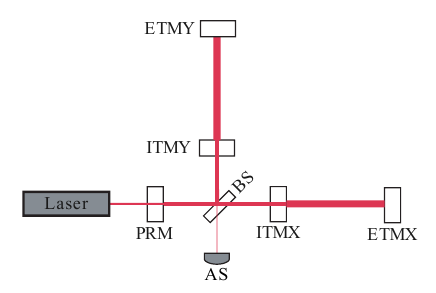
\includegraphics[width=0.6\columnwidth]{figures/ligo/ligo-schematic.png}} 
 \end{center}
\caption{\label{fig:ligo}Schematic of interferometric detectors, like LIGO.}
\end{figure}
%
Interferometric detectors like LIGO comprise of two laser cavities oriented 
orthogonal to each other. The mirrors at either end of each cavity are free to move 
in the horizontal direction, i.e. locally parallel to the surface of the Earth. 
In this restricted direction, for small fluctuations, these mirrors can be
considered as {\it freely-falling} to a good approximation.
The length of the arm cavities largely determines the amount of power stored
in the cavity. 
%
When plus (or cross) polarized gravitational waves pass through, they expand 
one cavity and contract the other, simultaneously, during half of their period,
and vice-versa during the other half. As a result, the difference of the cavities'
lengths (or the differential length) fluctuates, causing a differential fluctuation
in the laser power stored in each cavity. 
% 
Therefore, the effect of incoming gravitational radiation is converted to 
fluctuations of the laser power stored in two spatially orthogonal laser cavities.

Let us consider the schematic in Fig.~\ref{fig:ligo}. The laser source is 
depicted as a rectangle on the most left. The light from it travels through 
the {\it power recycling mirror} (PRM) and reaches the {\it beam 
splitter} (BS). The power recycling mirror reflects back the light 
that leaks out of the cavities in the arms, and in this sense {\it recycles}
the lost laser power. 
The beam splitter splits the main beam into two beams, one that travels along 
the $x$ arm and the other along the $y$ arm. Along the $x$ arm, the {\it end 
test-mass mirror} (ETM-X) and the {\it input test-mass mirror} (ITM-X) form a 
resonant {\it Fabry-Perot} cavity. Similarly for the $y$ arm.
The beams that finally come out of the the two cavities interfere at the beam
splitter and the interference pattern is recorded at the {\it dark port} (DP)
photodiode. This is called so because the two cavities are aligned in a way 
which ensures that the beam coming out of the $x$ arm interferes destructively
with that coming out of the $y$ arm, and hence in the absence of 
gravitational waves the port recording the interference pattern will be 
dark~\footnote{Initial LIGO was aligned at the dark fringe. However, in Advanced
LIGO a DC readout scheme will be used at the output port, 
in order to reduce the readout noise. 
This scheme is sensitive to the light power at the DP.
If the alignment was exactly on a dark fringe then any change in 
the arm lengths would only increase the light at the dark port, and we
would be unable to determine the direction in which the test-mass mirrors were
moving from DC readout. Therefore, the alignment in Advanced LIGO will be
slightly off the dark fringe}.
% 
Finally, a new addition to the Advanced LIGO optics topology is the {\it signal
recycling} (SR) mirror. It sends the signal coming out the dark port back into 
the arm cavities.
The optical system composed of the SR cavity and the arm
cavities forms a
composite resonant cavity, whose resonances and quality
factors can be controlled by the position and
reflectivity of the SR mirror. 
Near its resonances, the detector can gain sensitivity. 
% 
In what follows we discuss the effect of gravitational radiation on 
interferometric detectors, and some of the design choices involved.


Let us consider a $+$-polarized gravitational wave propagating in the 
$z-$direction, with the two arms of the detector along the $x$ and $y$ directions.
We can write down the spacetime metric in the TT gauge at the
location of the detector as
%
\begin{equation}
 \D s^2 = -\D t^2 + (1+h_+)\D x^2 + (1-h_+)\D y^2 + \D z^2.
\end{equation}
% 
% following the discussion in Sec.~\ref{sec:gravitational_radiation}. 
The LIGO 
cavity length is such that it ensures that the time taken by light to travel 
back and forth in it is much smaller comared to the time scale of variations in
$h_+$. Therefore, the time taken by light to make a round-trip between the end
test masses in the $x$ cavity 
% 
\begin{equation}
 t_x \simeq 2L_x (1 + \frac{1}{2}h_+),
\end{equation}
% 
where $L_x$ is the equilibrium length of the $x$ cavity in absence of 
gravitational waves. Here, we have expanded $\sqrt{1+h_+}$ as a Taylor series
and approximated it by keeping terms up to linear order. 
It follows that the light travel time for a round trip in 
the $y$ cavity is
% 
\begin{equation}
 t_y \simeq 2L_y (1 - \frac{1}{2}h_+).
\end{equation}
% 
As the two cavities share the laser source, the same light wavefront will 
return at the beam splitter at different delays in the $x$ than the $y$ cavity. 
Therefore, the change in the phase of the returning light would manifest as a 
phase difference $\delta\phi$ given by
% 
\begin{align}
 \delta\phi &= \Omega_L (t_x - t_y), \\ \nonumber
 &= 2 L\, \Omega_L\,\, h_+ = \dfrac{4\pi L}{\lambda_L}\,h_+,
\end{align}
where $\Omega_L$ ($\lambda_L$) is the frequency (wavelength) of the laser 
light, and we have assumed that $L_x = L_y$ and replaced them with $L$. 


The measurable change in phase $\delta\phi$ is directly 
proportional to the length of the cavities, or the {\it arms} of the detector.
As we aim to observe gravitational wave signals from 
astrophysical sources, which are far enough that the incident signal is
expected to be very weak, this motivates that the two arms be made as 
long as possible before practical considerations become prohibitive.
% 
% In each arm, the end and input test-mass mirrors, $ETM\{X,Y\}$ and 
% $ITM\{X,Y\}$, form a resonant {\it Fabry-Perot} cavity. The end mirrors are 
% highly polished and stabilized in order to maximize their reflectivity. 
% The laser light forms a standing wave in these cavities, and accumulates power.
In addition, the reflectivity of the end mirrors (in each arm) is carefully
controlled, so that each 
wavefront bounces back and forth several times before exiting the cavity and 
interfering at the beam splitter. The net benefit is similar to increasing the
effective length of each arm $L$ by a factor of $\sim 200$ (for LIGO). 
% 
In addition to the layout in Fig.~\ref{fig:ligo}, there are a number of
optical, electronic, mechanical, and electromagnetic sub-systems of LIGO 
detectors that are designed to maximize the sensitivity and efficiency of the detectors.
A treatment of their details is out of the scope of this dissertation, and we
refer the reader to~\cite{lrr-2011-5,Harry:2010zz} for a more technical overview.
% is an {\it output mode
% cleaner} in the path of the output beam between the BS and the DP. The cross 
% section of this beam can be decomposed as Hermite-Gaussian modes, and only the 
% lowest order mode contributes to the readout at the DP. All higher modes
% instead only add to the noise at the readout port, and the output mode 
% cleaner 



\section{Dominant Noise Sources}\label{sec:ligo_noise}

We define the strain signal, $s$, to be the relative change in the length 
of the two arms of the interferometer
% 
\begin{equation}
 s(t) = \dfrac{\Delta L_x - \Delta L_y}{L}.
\end{equation}
% 
The signal $s(t)$ can be written as the sum of two components, (i) the actual
differential arm length change induced by the incident gravitational wave 
$h(t)$ (if present), and (ii) the sum of various noises, $n(t)$, that affect 
the measurement of the difference in the arm lengths $\Delta L$. 
%
As the goal of LIGO is to measure remarkably small length changes, several
sources of noise that propagate to the measurement of $s(t)$ become 
consequential. A few intrinsic to the instrument include the brownian motion
noise in mechanical systems, lossy optics, cross-talk in electromagnetic
systems, noise in control electronics, etc. Additionally, there are noise 
sources in the environment of the detectors, such as wind and ground motion,
fluctuations in the Newtonian gravity due to changes in atmosphere or ground
density, electric coupling from nearby power lines etc. 
%
It is therefore a challenging task to categorize these sources and reduce the
noise to the best extent possible.


Gravitational wave searches in LIGO data are affected by the {\it power
spectral density} of all the noise sources combined. The fundamental noise 
sources that limit the sensitivity of the interferometer in different frequency
ranges are:
% 
\begin{enumerate}
 \item Seismic noise:
 The motion of the ground, whether it be due to earthquakes or due to human 
 activity, couples mechanically to suspended test-mass mirrors at both the ends
 of each arm. This coupling leads to fluctuation in their vertical and horizontal
 position, directly affective the measurement of differential arm length.
 The suspension of mirrors as pendula acts as a low pass filter for seismic
 motion. There are active systems in place as well that sense ground motion and 
 feed the information back to cancel its effect. Seismic noise affects the 
 sensitivity of the detectors at frequecies  $< 40$~Hz.
 \item (Suspension) thermal noise:
 Any physical degree of freedom has an expected energy that depends on the temperature,
 leading to thermal noise in the observations related to that degree of freedom.
 The leading source of thermal noise is the molecular Brownian motion in the
 mirror suspension wires, and in the surface of the mirror. Thermal noise is 
 a low frequency noise that falls off inversely with (the square of) frequency. 
 It dominates  the detector sensitivity in the range $\sim 40-150$~Hz.
 \item Photon shot noise:
 During operation, the interferometer is locked 
 with the optical fields from the two arms interfering destructively at the
 beam splitter, or in other words at a {\it dark fringe}. The number of photons
 that arrive at the readout will be directly proportional to any incident
 gravitational wave signal. The arrival times of the photons at the DP 
 follow Poissonian statistics. Therefore the counting of the number of
 photons that arrive in a given interval of time, $\mathcal{N}$, will have an 
 inherent uncertainty proportional to $\sqrt{\mathcal{N}}$. However, the {\it signal}
 contained in the laser light increases with $\mathcal{N}$, and therefore the 
 signal-to-noise ratio is $\propto \sqrt{\mathcal{N}}$.
 %
 In frequency domain, the shot noise has a flat (or {\it white}) spectrum. 
 However, the arms of the interferometer act as a filter and amplify the effect
 of the shot noise on our ability to measure the incident gravitational wave
 with increasing frequency. As a result, this noise source dominates over all
 others at $f\gtrsim 1$~kHz.
\end{enumerate}
% 
We refer the reader to~\cite{Saulson:1995zi} for a detailed treatment of these
noise sources, which is out of scope of this dissertation. 

Apart from these continuous noise sources, there is another class of noise 
that plagues our ability to systematically extract signals embedded in detector
data called {\it glitches}. Glitches are transient by definition, and have a 
variety of frequency spectrum and sources. More importantly, if not correctly 
identified with their cause, they could be unpredictable. For instance, the 
falling of a 
heavy object could shake optics and lead to a sharp rise in the noise level
in the differential arm length output. There are mechanisms being developed to 
identify and classify glitches in Advanced LIGO and Virgo, within the Detector
characterization group. There are also algorithms in place that allow search 
methods to differentiate between signals and glitches based on their frequency
spectrum and evolution.


% % This section is completely un-necessary
% \section{Calibration of LIGO}\label{sec:ligo_calibration}
% \begin{figure}
%  \begin{center}
%   \scalebox{1}{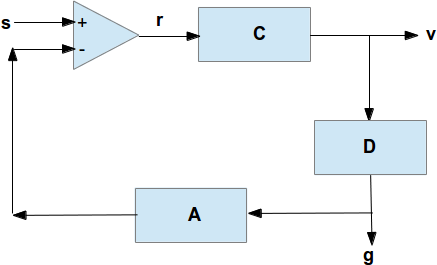
\includegraphics[width=0.6\columnwidth]{figures/ligo/ligo-control-loop.png}} 
%  \end{center}
% \caption{\label{fig:ligo_calibration}Model for the control loop of the LIGO
% length sensing and control system.}
% \end{figure}
% 
% The signal recorded at the output port $v(t)$ is proportional to the effect of 
% the differential motion of the mirrors in the two arms of the interferometer.
% This signal is itself used in a control loop to further stabilize the free-falling
% masses by actuating on them. Therefore the effect of the gravitational waves alone, 
% $s(t)$, has to be decoded from $v(t)$ by understanding this control loop.
% 
% Let us model this length sensing control loop as in
% Fig.~\ref{fig:ligo_calibration}. All the blocks symbolize the transfer function
% of a particular logical block, which is the ratio of its output to its input.
% All quantities hereafter will be in frequency domain, while the transfer 
% functions themselves could be slowly varying in time as well. 
% Block $C$ denotes the 
% length sensing function. It measures the response of the arm cavities to 
% gravitational waves. Block $D$ converts the output of block $C$, i.e. the 
% fluctuation in the differential arm length into a control signal that is sent
% to block $A$. Block $A$ is the {\it actuation} function that reacts to the 
% control signal and actuates upon the suspended masses in a way so as to 
% stabilize them. 
% 
% We calculate the transfer function $G$ between the readout and the actual 
% gravitational wave signal as
% %
% \begin{equation}
%  \begin{split}
%   v = C\, r ;\hspace{5mm} g &= D\, v = CD\, r ;\hspace{5mm} r = s - A\, g = s - CDA\, r, \\
%   &\Rightarrow G \defeq \dfrac{s}{v} = \dfrac{1 + CDA}{C}.
%  \end{split}
% \end{equation}
% % 
% The process of calibrating interferometer data therefore involves measuring 
% the aforementioned transfer functions to high accuracy and using them to obtain 
% the final data channel containing the possible gravitational wave signal.



\section{Detector response to Gravitational wave polarizations}\label{sec:ligo_response}
\begin{figure}
 \begin{center}
  \scalebox{1}{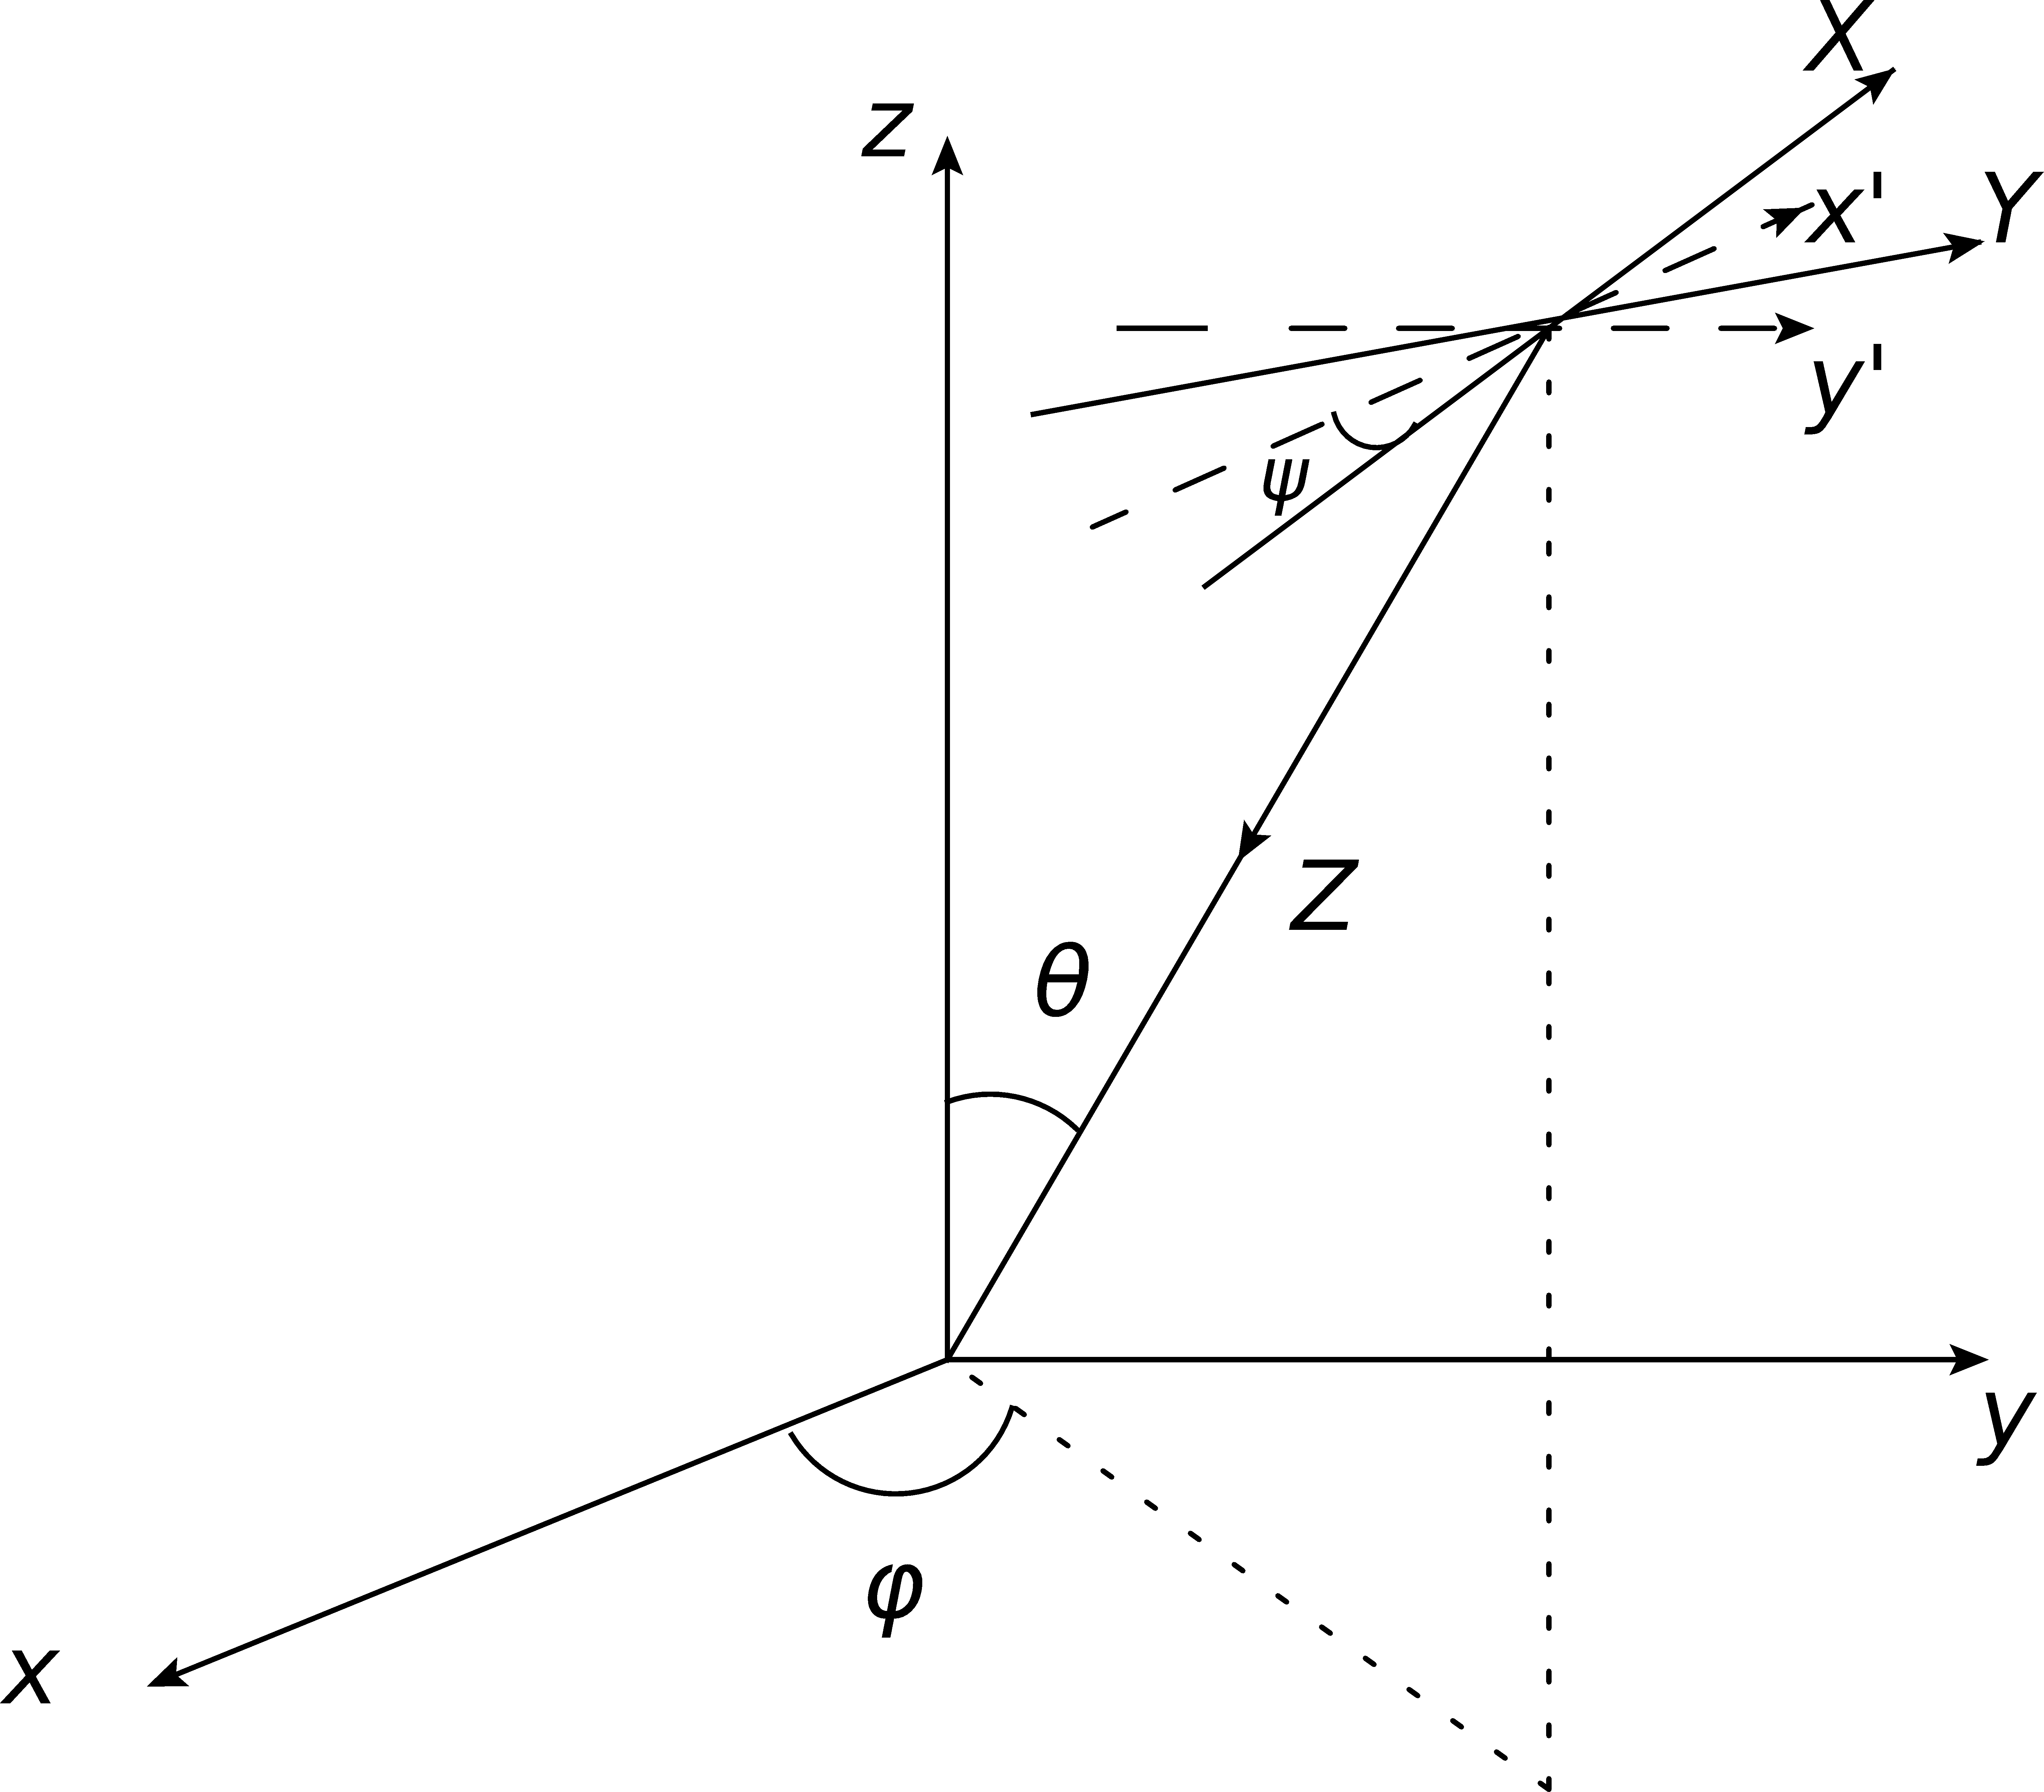
\includegraphics[width=0.6\columnwidth]{figures/ligo/radiation-detector-frame.png}} 
 \end{center}
\caption{\label{fig:radiation_detector_frames}
The Euler angles $\{\theta,\phi,\psi\}$ to go from teh gravitational 
wave propagation frame to the detector frame.}
\end{figure}

We start with defining the radiation frame which has its $x-y$ plane in the 
plane of the sky if one is looking towards the source. The line connecting the 
source and the detector defines its $z-$axis. Therefore we can determine the 
polar angles $(\theta,\phi)$ that point along the $z-$axis of the 
radiation frame. Finally, we denote the angle between the $x-$axis of the 
radiation frame and the plane made by joining the $x-$arm of the detector and
the $z-$axis of the radiation frame. The detector frame is intuitively defined
by defining the $x$ and $y$ axes along the two arms with the $z-$axis coming
out of the plane of the detector on Earth.

It can be shown that the polarization amplitudes in the radiation frame depend 
on the {\it inclination} angle $\iota$ between the orbital (or total) angular 
momentum of the binary and the line of sight from the detector to the source
as~\cite{SathyaSchutzLRR}
% 
\begin{equation}\label{eq:h_inclination}
 h_+ = \frac{1}{2}(1 + \cos^2\iota)\,h_0\cos\Phi(t); \hspace{10mm} h_\times = \cos\iota\,h_0\sin\Phi(t).
\end{equation}
%
$h_0$ is an overall amplitude that varies slowly in time compared to the 
instantaneous gravitational wave phase $\Phi(t)$. 
In the radiation frame the tensorial metric perturbation can be written as 
(bold fonts indicate tensors or vectors with indices suppressed)
\begin{equation}
 {\bf h} = h_+{\bf e_+} + h_\times{\bf e_\times}
\end{equation}
% 
where the basis tensors are defined as
% 
\begin{equation}
 {\bf e_+}\defeq {\bf e^R_x}\otimes {\bf e^R_x} - {\bf e^R_y}\otimes {\bf e^R_y}; \hspace{10mm}
 {\bf e_\times}\defeq {\bf e^R_x}\otimes {\bf e^R_y} + {\bf e^R_y}\otimes {\bf e^R_x},
\end{equation}
% 
with ${\bf e^R_x}$ and ${\bf e^R_y}$ being unit vectors along the $x$ and $y$ 
axes of the radiation frame. Next we define the {\it detector tensor}, which 
can be thought of as the projection tensor for the detector, as
% 
\begin{equation}
 {\bf d} \defeq L({\bf e^D_x}\otimes {\bf e^D_x} - {\bf e^D_y}\otimes {\bf e^D_y}),
\end{equation}
% 
where ${\bf e^D_x}$ and ${\bf e^D_y}$ are unit vectors along the $x$ and $y$ 
axes of the detector frame, and they point along the direction of the arms from 
the central beam splitter. $L$ is the length of each arm of the interferometer. 
The change in length of the arms $\delta L(t)$ can therefore be obtained as the
scalar product between the ${\bf h}$ tensor and the detector tensor, i.e.
% 
\begin{equation}
 \delta L(t) = {\bf d}\cdot {\bf h} \defeq d_{ij}h^{ij}
\end{equation}
% 
This allows the strain produced in the arms to be written as
% 
\begin{equation}\label{eq:h_strain_antenna}
 h(t)\defeq\frac{\delta L}{L} = F_+(\theta, \phi, \psi) h_+ + F_\times(\theta, \phi, \psi) h_\times,
\end{equation}
where the functions $F_+$ and $F_\times$ can be found using the geometry in
Fig.~\ref{fig:radiation_detector_frames} as the scalar product of the basis tensors
${\bf e_+}$ and  ${\bf e_\times}$ with the detector tensor~\cite{SathyaSchutzLRR},
% 
\begin{equation}\label{eq:fpluscross}
 \begin{split}
  F_+ &= \frac{1}{2}(1 + \cos^2\theta)\cos(2\phi)\cos(2\psi) - \cos(\theta)\sin(2\phi)\sin(2\psi), \\
  F_\times &= \frac{1}{2}(1 + \cos^2(\theta))\cos(2\phi)\sin(2\psi) + \cos(\theta)\sin(2\phi)\cos(2\psi).
 \end{split}
\end{equation}
These two functions are called the {\it antenna patterns} of the detector, 
and they define the response of the detector to incoming gravitational 
radiation governed purely due to the relative geometry between the source and 
the detector itself. Finally, collecting Eq.~\eqref{eq:h_inclination} and
Eq.~\eqref{eq:h_strain_antenna} we can write the strain $h(t)$ seen by the 
detector as
% 
\begin{equation}
 h(t) = F_+ h_+ + F_\times h_\times = \mathcal{A} h_0 \cos(\Phi(t) - \Phi_0),
\end{equation}
% 
where $\Phi(t)$ has the same meaning as in Eq.~\eqref{eq:h_inclination}, and
% 
\begin{equation}
\begin{split}
 \mathcal{A} &\defeq \left(\left(\frac{1}{2}F_+(1+\cos^2\iota)\right)^2 + \left(F_\times\cos\iota\right)^2\right)^{1/2}, \\
 \Phi_0 &\defeq \tan^{-1}\left( \frac{2F_\times\cos\iota}{F_+(1+\cos^2\iota)}\right),
\end{split}
\end{equation}
% 
are combinations of the antenna patterns and the inclination angle folded 
into a constant amplitude and phase change. 

